\chapter{Arquitectura del sistema}
\label{cap:arquitectura}
Para conseguir que los distintos módulos que integran el sistema trabajen de forma conjunta es necesario establecer una arquitectura que permita la comunicación eficiente entre ellos así. Para coordinar el trabajo de los distintos módulos que componen el sistema se ha empleado ROS (\textit{Robot Operating System}) \cite{ros} un \textit{framework} orientado a el desarrollo de software para robots ampliamente extendido en la comunidad robótica. En el paradigma de ROS el código se estructura en nodos independientes que se comunican entre ellos a través de tópicos (mensajes que un nodo difunde de forma general a los demás nodos y cualquiera lo puede leer) y servicios (peticiones de un nodo particular a otro).

Esto permite desarrollar cada componente del sistema de forma independiente y comunicarlos entre ellos mediante una interfaz común. Esto permite encapsular el código, lo que aumenta la reusabilidad y la robustez de cada módulo, independiente del resto de módulos que les rodeen.

A continuación se explicará más detalladamente los distintos nodos que componen la arquitectura:
\begin{itemize}
	
	\item \textbf{Simulador:} En la arquitectura propuesta el entorno de simulación empleado, Flightgoogles, se comporta como un nodo adicional. Este nodo constituye el interfaz de comunicación entre el aeronave simulada y el entorno simulado,
	el cual publica datos sobre el estado del aeronave como su posición y orientación, las imágenes de las cámaras simuladas y la posición de las esquinas de las puertas en las imágenes obtenidas. Asimismo, recibe los comandos de control enviados al aeronave.
	 
	\item \textbf{Estimación de estado.} Este modulo se encarga de completar la estimación de estado del aeronave, empleando la información temporal sobre los cambios de pose del aeronave. Además proporciona esta información a través de mensajes estándar al resto de los módulos de la arquitectura.
	
	\item \textbf{Percepción.} El simulador provee las imágenes, tomadas por las cámaras, del entorno simulado. En estas imágenes aparecen las puertas del circuitos con un indicador del número de puerta, así como las posiciones de las esquinas de las puertas en las imágenes tomadas. Conociendo los parámetros de la cámara y las dimensiones de las puertas se puede extrapolar la posición de las puertas respecto a la cámara. El modulo de percepción se encarga de enviar las posiciones aproximadas de las distintas puertas del circuito e ir actualizando estas estimaciones a medida que el aeronave avanza a través del circuito.
	
	\item \textbf{Generador de trayectorias.} Una vez conocida la posición del aeronave en el circuito y las posiciones aproximadas de las puertas con respecto a el aeronave se genera la trayectoria que debe seguir el aeronave para pasar a través de las puertas de la forma más rápida posible sin colisionar con el entorno. Para poder actualizar la trayectoria de forma rápida con un coste bajo computacional se divide este trabajo en dos módulos:
	
	\begin{itemize}
		\item \textbf{Trayectoria a largo plazo}: Obtiene las posiciones de las puertas provistas por el módulo de percepción y genera el recorrido tridimensional completo que debería realizar el cuadricóptero. 
		
		\item \textbf{Trayectoria a corto plazo}: Recibe la trayectoria a largo plazo y la evalúa en un corto horizonte temporal respecto a la posición actual del aeronave. Dentro de este horizonte se genera la trayectoria de control óptima a seguir. Este módulo también se encarga de evaluar la trayectoria actual a lo largo del tiempo y enviar las consignas de posición, velocidad y aceleración al controlador.
	\end{itemize}
	
	\item \textbf{Controlador:} El módulo del controlador recibe el estado actual del aeronave provisto por el modulo de estimación y la referencias provistas por el módulo trayectoria a corto plazo. Con esto genera las acciones de control que se envían al módulo del simulador.
	
\end{itemize}

\begin{figure}[htb!]
	\centering
	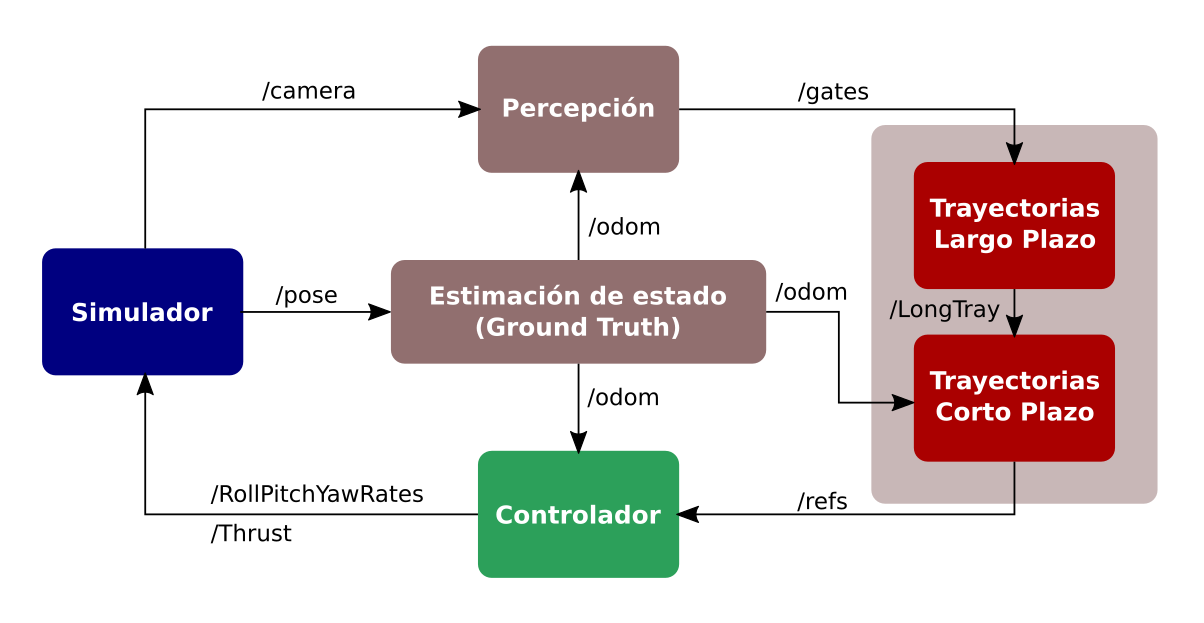
\includegraphics[width=\textwidth]{imagenes/Arquitectura}
	\caption{Diagrama de la arquitectura empleada con los tópicos principales}
	\label{Arquitectura}
\end{figure}


\section{Detalles de implementación}

Todos los algoritmos desarrollados se han implementado en C++17 haciendo uso tanto de las librerías estándar como de las librerías estándar de ROS . Además se ha hecho uso de algunas librerías específicas como OpenCV 4.0 para el tratamiento de las imágenes, así como Eigen3 para computar las operaciones matriciales requeridas por los algoritmos implementados. A continuación, se explicarán algunos detalles de implementación relevantes de los distintos módulos.

\subsection{Módulo de control}

Para facilitar el ajuste de las ganancias de los distintos controladores se ha empleado la librería de ROS \textit{dynamic reconfigure}. Esta librería permite variar el valor de distintos parámetros en tiempo de ejecución, lo que facilita enormemente el ajuste fino de los parámetros de los controladores. 
\begin{figure}[htb!]
	\centering
	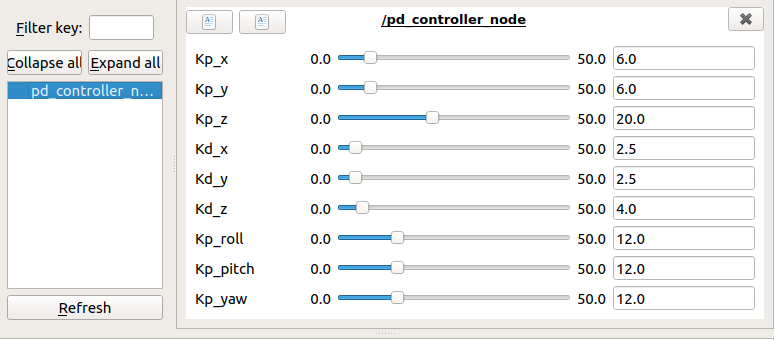
\includegraphics[width=0.9\textwidth]{imagenes/Rqt}
	\caption{Ventana de configuración \textit{dynamic reconfigure}}
	\label{waypoints:circuito}
\end{figure}




\subsection{Módulo de generación de trayectorias}

Dado que las dos trayectorias generadas, la de corto y la de largo plazo, se generan empleando \textit{splines} se ha unificado el algoritmo de generación en una clase común a ambos módulos. Aunque al comienzo del proyecto se empleo una implementación propia de estos algoritmos, finalmente se ha optado por emplear la implementación realizada por la ETHZ (disponibles para la comunidad robótica en \url{https://github.com/ethz-asl/mav_trajectory_generation}) debido a que alcanzaban una mayor eficacia en la generación de las mismas.

Adicionalmente, debido a que el módulo generador de trayectorias a corto plazo es el encargado también de generar las referencias del controlador ha sido necesario paralelizar la generación de las trayectorias y la evaluación de las mismas a lo largo del tiempo. Es por eso que se ha separado la computación en dos hilos diferentes: un hilo principal que se encarga de muestrear la trayectoria generada a una alta frecuencia (100 Hz) y de enviar las referencias al controlador y un hilo secundario que se encarga de generar la siguiente trayectoria a corto plazo a seguir.

%\tb{\Large Pequeña imagen de los hilos}




